%Dit is een verkorte versie, doel is om alles op 1/2 pagina's te krijgen

\chapter{Bedrijfsachtergrond}
\label{hoofd:bedrijfsachtergrond}
\textbf{Voor het beantwoorden van de hoofdvraag richt dit onderzoek zich voornamelijk op de organisatie en welke maatregelen er getroffen zijn om risico's af te schermen. Het schept extra inzicht om hiervoor te kijken naar hoe de organisatie is ingericht en welke invloeden dat heeft op de omgang met financiële vermogenswaarden.}

\medskip
\noindent
In 1995 richtten huidig CEO J. (Jan) Kaptijn en wijlen C. (Chris) Goos Seafood Connection (hierna als afkorting: SFC) op. De oprichters kwamen met het innovatieve idee om een geselecteerd assortiment visproducten aan te bieden over de hele wereld zonder zelf ook maar een enkele visverwerkingsband te moeten aanschaffen. Seafood Connection werkt nauw samen met landen over de hele wereld om lokaal visproducten aan te kunnen bieden met een hoge kwaliteitsstandaard. SFC kan deze hoge standaard garanderen door contacten van het bedrijf zelf, grondige controles uit te voeren bij de leveranciers en het productie- en verwerkingsproces. Hoge Europese standaarden als IFS, BRC, MSC en HACCP dicteren en nauwlettende werkwijze. \citep{sfcreglement}

Seafood Connection is een handelsbedrijf in diverse diepvries visproducten met daarnaast in beperkte mate doorstroom van eigen goederen met een eenvoudig, technisch omzettingsproces \citep{aoibsfc}. 


\vfill
\begin{center}
  \makebox[\textwidth]{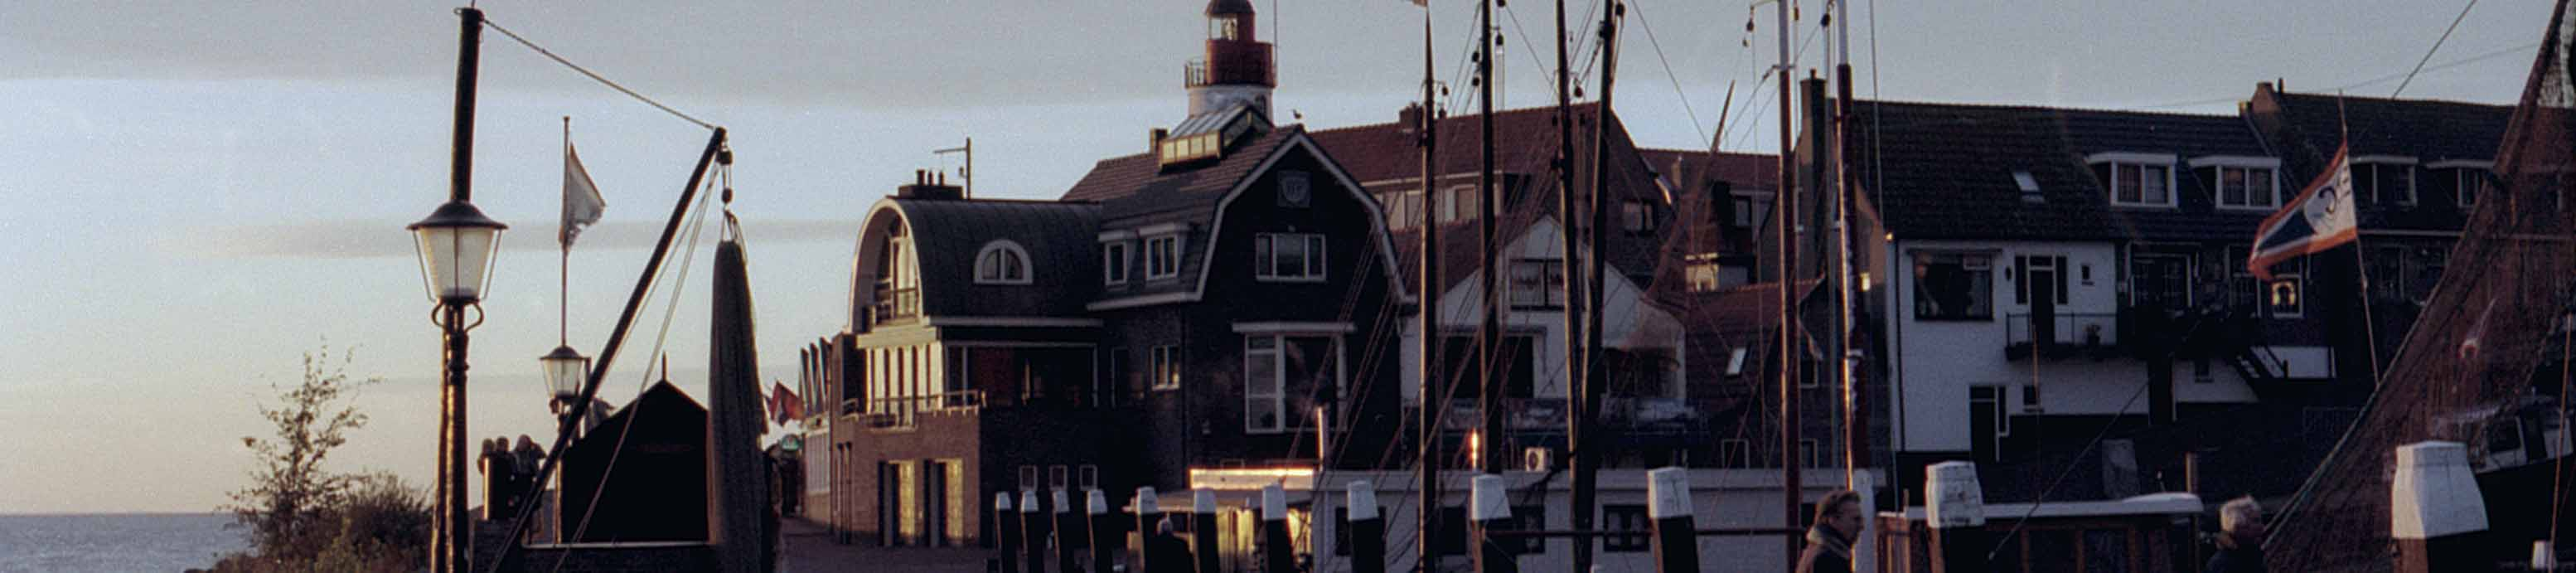
\includegraphics[width=1.09\paperwidth]{scn210}}
\end{center}

\newpage
\noindent
Voor de verschillende bedrijfsactiviteiten fungeert Seafood Connection als:

\begin{enumerate}
    \item Handelsbedrijf dat hoofdzakelijk aan andere bedrijven levert;
    \item In beperkte mate een productiebedrijf met homogene massaproductie;
    \item Commissie op verkopen aan derden: in zeer beperkte mate dienstverlening aan derden.
\end{enumerate}

Seafood Connection is vijftig gemotiveerde werknemers sterk. Het kantoor op Urk vervult alle bedrijfsfuncties grotendeels op één locatie; er zijn enkele medewerkers werkzaam bij een klein, lokaal productieproces, namelijk bij de zagerij van Coldstore Urk waar een groot deel van de voorraad van SFC zich bevindt. De organisatie heeft vier niveaus: het managementteam (MT) dat de strategie formuleert, de unitmanagers (UMO) die hun afdelingen aansturen, managers die het aanspreekpunt zijn voor hun deelprocessen in de verschillende afdelingen, én assistants die de afdelingen ondersteunen met verschillende werkzaamheden. SFC is een \gls{lsorganisatie} met een gedeelde P-, G-, en M-indeling opgedeeld in de afdelingen: inkoop, opslag, verkoop, finance, ICT and production, HRM, compliance, en marketing verdeeld over vier segmenten: wholesale, retail, industry, en group companies. \citep{quickscan}

In 2013 kocht het Japanse Maruha Nichiro de meerderheid van Seafood Connection Holding. SFC hoopt met deze samenwerking te kunnen profiteren van de kennis en middelen van Maruha Nichiro, die naast de verkoop van visproducten het doel hebben om de hele waardeketen van de visindustrie te domineren. Onderstaande figuur geeft een idee van de geografische reikwijdte van het bedrijf. In blauw de kantoren van SFC, in rood de vestigingen van moederbedrijf Maruha Nichiro. \citep{sfcwebsite,Visserijnieuws}

\begin{figure}[!h]
    \centering
    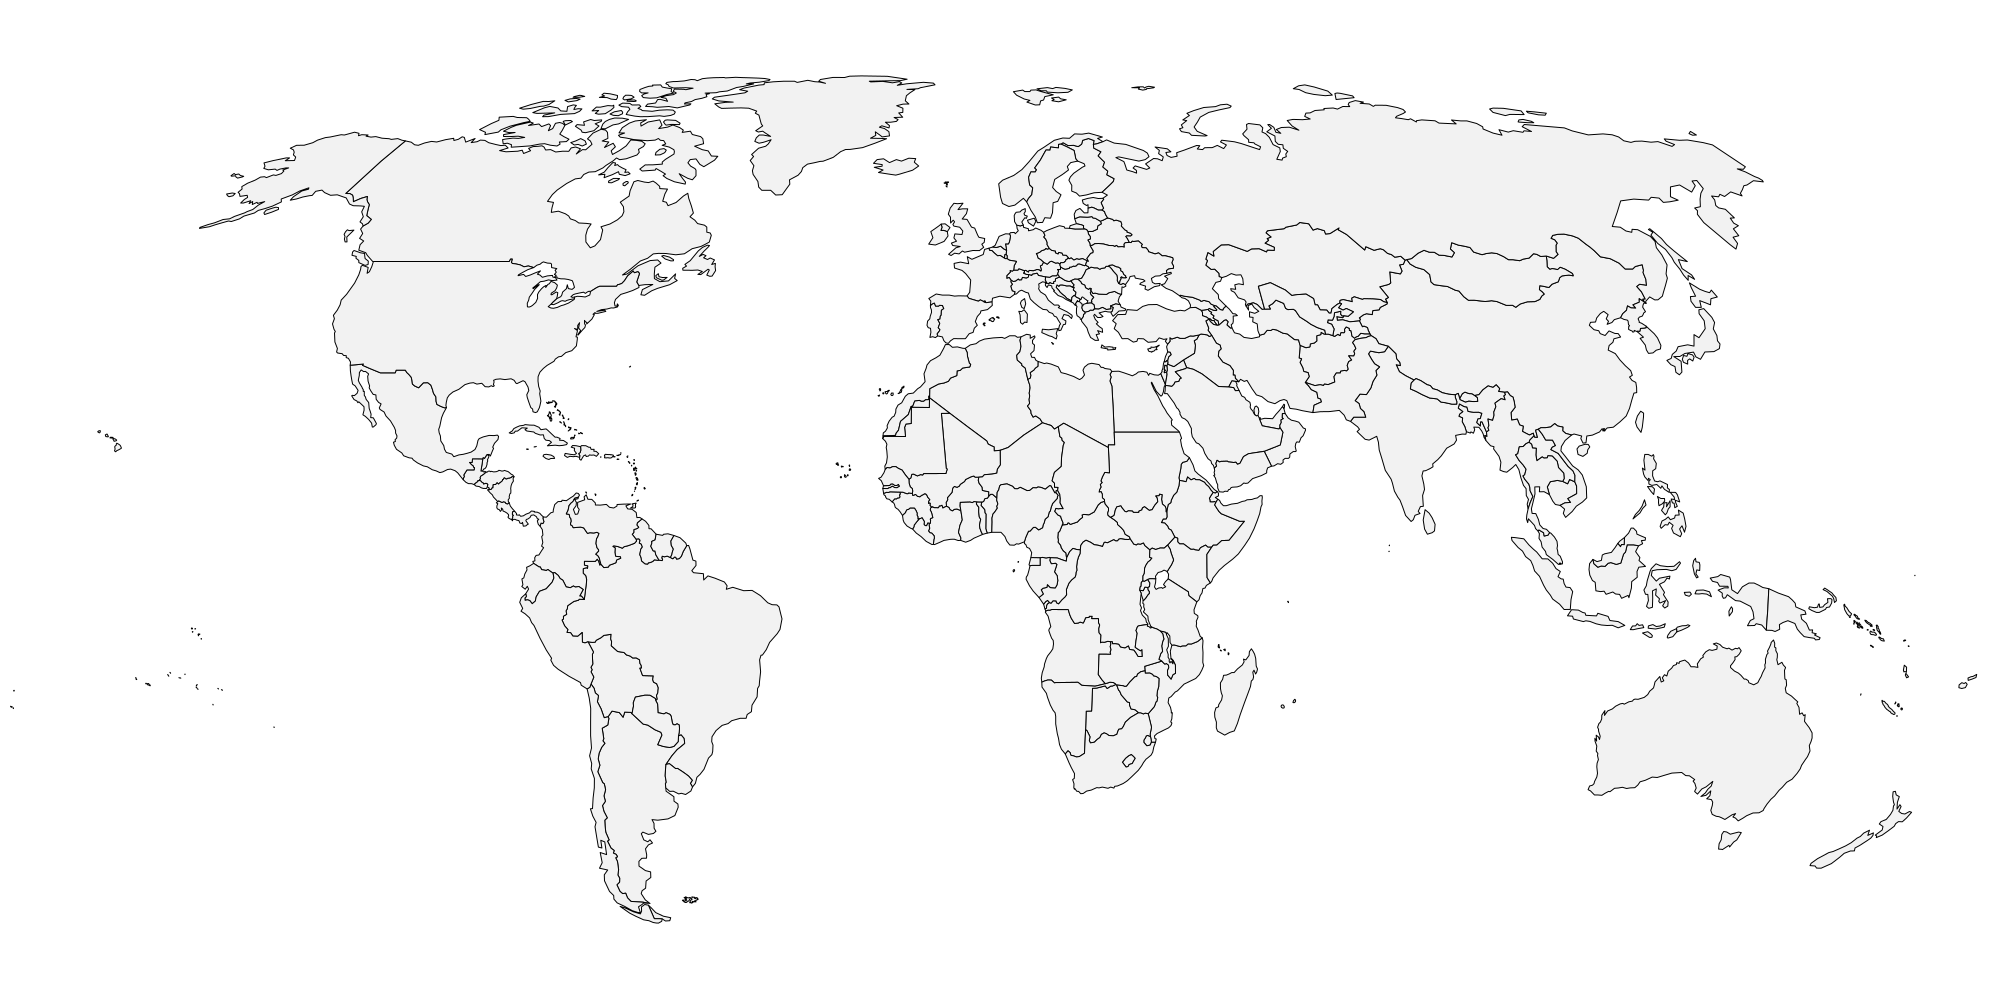
\includegraphics[width=0.9\textwidth]{kaart}
    \caption{De kantoren van SFC en Maruha \citep{sfcwebsite}}
    \label{fig:kantorensfc}
\end{figure}

De missie van Seafood Connection is om het volgende te anticiperen: klantbelangen, de behoefte aan duurzame visproducten, en nieuwe trends. De onderneming wil dit realiseren door nieuwe partners te verkrijgen in cruciale markten in Europa, Amerika en Azië. Tevens worden nieuwe keteninnovaties verkregen door fusies en overnames in de visindustrie. \citep{sfcwebsite}

\label{beschr:activiteiten}
SFC heeft een belangrijke kritische succesfactor wat het moeilijk maakt voor nieuwkomers op de markt om Seafood Connection te verdrijven. Het is namelijk enorm kapitaalintensief om op grote schaal visproducten af te zetten. Bedrijven op de internationale vismarkt staan onder grote liquiditeitsdruk. Deze druk komt onder andere voort uit het feit dat vishandelaren de inkopen dikwijls vooruitbetalen. Dit heeft tot gevolgd dat de crediteurenpositie binnen Seafood Connection laag is, maar er moet aan het begin van het handelsproces dus meteen al betaald worden. Het proces tussen inkoop, opslag, verkoop en daadwerkelijk ontvangst van de verkoopfactuur bedraagt afhankelijk van het product tussen de vier en zes maanden. Dit risico is schematisch weergegeven in figuur \ref{fig:liquiditeitsrisico}. 

Een MKB onderneming kan geen tonnen vooruit financieren omdat hun financiële positie dat niet toelaat. Al zou het mogelijk wezen om dit geld te kunnen lenen, dan zijn de rentekosten aanzienlijk omdat het financieringsrisico voor de bank hoog is. Een klein bedrijf kan hierdoor tot wel 8\% rente betalen op het geleende krediet. Dit terwijl SFC een brutomarge heeft van 8\%, het MKB bedrijf zal dus nooit competitiever zijn dan SFC. Hierbij komt ook dat Seafood Connection de visproducten op basis van grote volumes koopt en hiermee een gunstige onderhandelingspositie heeft. \citep{quickscan}

\begin{figure}[!h]
    \centering
    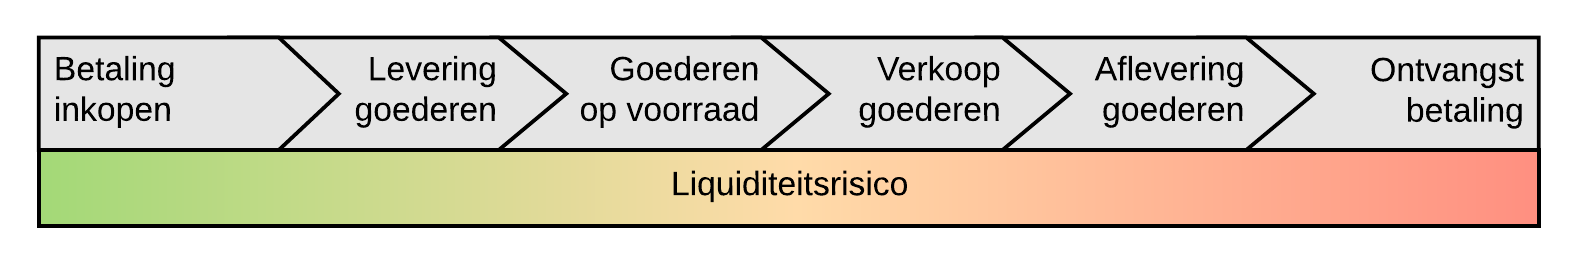
\includegraphics[width=1\textwidth]{liquiditeitsrisico}
    \caption{Liquiditeitsrisico en druk op de schulden gedurende het bedrijfsproces}
    \label{fig:liquiditeitsrisico}
\end{figure}

Samenvattend bevindt SFC zich in een gunstige onderhandelingspositie en kan zo hard groeien juist doordat de onderneming zo groot is. Dit neemt niet weg dat een sterke organisatie onmisbaar is. De aard van de transacties, het schuiven van financiële vermogenswaarden en de unieke bedrijfsuitoefening dragen allemaal mee aan de complexiteit van de organisatie. De externe omgeving is de context van het centrale probleem. Om tot de juiste antwoorden en conclusies te komen is het belangrijk om uit te zoeken wat precies de vraag is en het probleem dat opgelost dient te worden.